\documentclass{cmc}

\begin{document}

\pagestyle{fancy}
\lhead{\textit{\textbf{Computational Motor Control, Spring 2024} \\
    Python exercise, Lab 4, NOT GRADED}} \rhead{Student \\ Names}

\section*{Student names: \ldots (please update)}

\textit{Instructions: Update this file (or recreate a similar one, e.g.\ in
  Word) to prepare your answers to the questions. Feel free to add text,
  equations and figures as needed. Hand-written notes, e.g.\ for the development
  of equations, can also be included e.g.\ as pictures (from your cell phone or
  from a scanner).  \textbf{This lab is not graded. However, the lab exercises
    are meant as a way to familiarise with dynamical systems and to study them
    using Python to prepare you for the final project.} This file does not need
  to be submitted and is provided for your own benefit. The graded exercises
  will have a similar format.}

\textit{The file \fileref{lab\#.py} is provided to run all exercises in Python. When
  a file is run, message logs will be printed to indicate information such
  as what is currently being run and and what is left to be implemented. All
  warning messages are only present to guide you in the implementation, and can
  be deleted whenever the corresponding code has been implemented correctly.}

\textit{In this lab, you will be modifying \fileref{lab4.py}, \fileref{network.py}
		and \fileref{simulation\_parameters.py}.}


\section*{Coupled firing rate neurons to model a swimming CPG segment}

\textit{The lab of today is based on networks of single/coupled firing rate neuron models with
  adaptation that describes the coarse-grained activity of a population of neurons. You will use similar models to build a controller in the zebrafish project. These models that were studied in the following papers:
  \begin{itemize}
  \item \href{https://journals.physiology.org/doi/full/10.1152/jn.00228.2011}{Seely, J., \& Chow, C. C. (2011). Role of mutual inhibition in binocular rivalry. Journal of neurophysiology, 106(5), 2136-2150.}
  \item \href{https://epubs.siam.org/doi/abs/10.1137/070705842}{Curtu, R., Shpiro, A., Rubin, N., \& Rinzel, J. (2008). Mechanisms for frequency control in neuronal competition models. SIAM journal on applied dynamical systems, 7(2), 609-649.}
  \end{itemize}
  This model can be used to study the generation of the swimming rhythm by the CPGs in fishes, such as the lamprey or the zebrafish, and the dependence on several biophysical parameters, such as input drive from the brain, excitatory and inhibitory weights, etc. }

\subsection*{Model equations}

The equations of a single firing rate unit modeling a single hemisegment oscillator that you will need to implement is described by the following pair of equations
\begin{equation}
    \begin{array}{lcl}
    \tau \dot{r} & = & -r + F(I + \alpha r - b a) \\
    \tau_a \dot{a} & = & -a + r, \\
    \end{array}
    \label{single_unit_eqn}
\end{equation}
where $r$ represents the firing rate of the neuron, and $a$ the firing rate adaptation (fatigue). The biophysical meaning of the parameters in system \ref{single_unit_eqn} is reported in Table \ref{table_par}, respectively. We assume that the system operates in the slow-fast regime, i.e. $\tau$ much smaller than $\tau_a$. This means that the neuron's spiking dynamics is faster than that of the firing adaptation, which is what is typically observed experimentally.

\begin{table}[h!]
\centering
\begin{tabular}{ l l }
 Parameter & Meaning \\
 $\tau>0$ & Neuron timescale \\
 $\tau_a>0$ & Adaptation timescale \\
 $b>0$ & Adaptation strength \\
 $\alpha>0$ & Self-excitation strength\\
 $I>0$ & Input current (i.e. from higher brain centers) \\
 $w$ & Coupling strength  ($w>0$=inhibitory connection, $w<0$=excitatory connection)
\end{tabular}
\caption{Biophysical meaning of the parameters of the firing rate network}
\label{table_par}
\end{table}

The function $F=F(x)$ in equation \ref{single_unit_eqn} is called gain function (also known as activation function, or transfer function), and it is the input-output non-linearity capturing the neural properties of the system. Here we will consider and study the role of three different types of gain functions (see Figure 1). We will consider a sigmoid gain
\begin{equation}
F(x)=F_{\lambda,\theta}(x)=\frac{1}{1+e^{\lambda (\theta-x)}},
\label{sigmoid_eq}
\end{equation}
a rectified linear unit (ReLu) gain
\begin{equation}
F(x)=max(x,0),
\label{ReLu_eq}
\end{equation}
and the square ReLu gain
\begin{equation}
F=\sqrt{max(x,0)}.
\label{SReLu_eq}
\end{equation}


\begin{figure}
	\centering 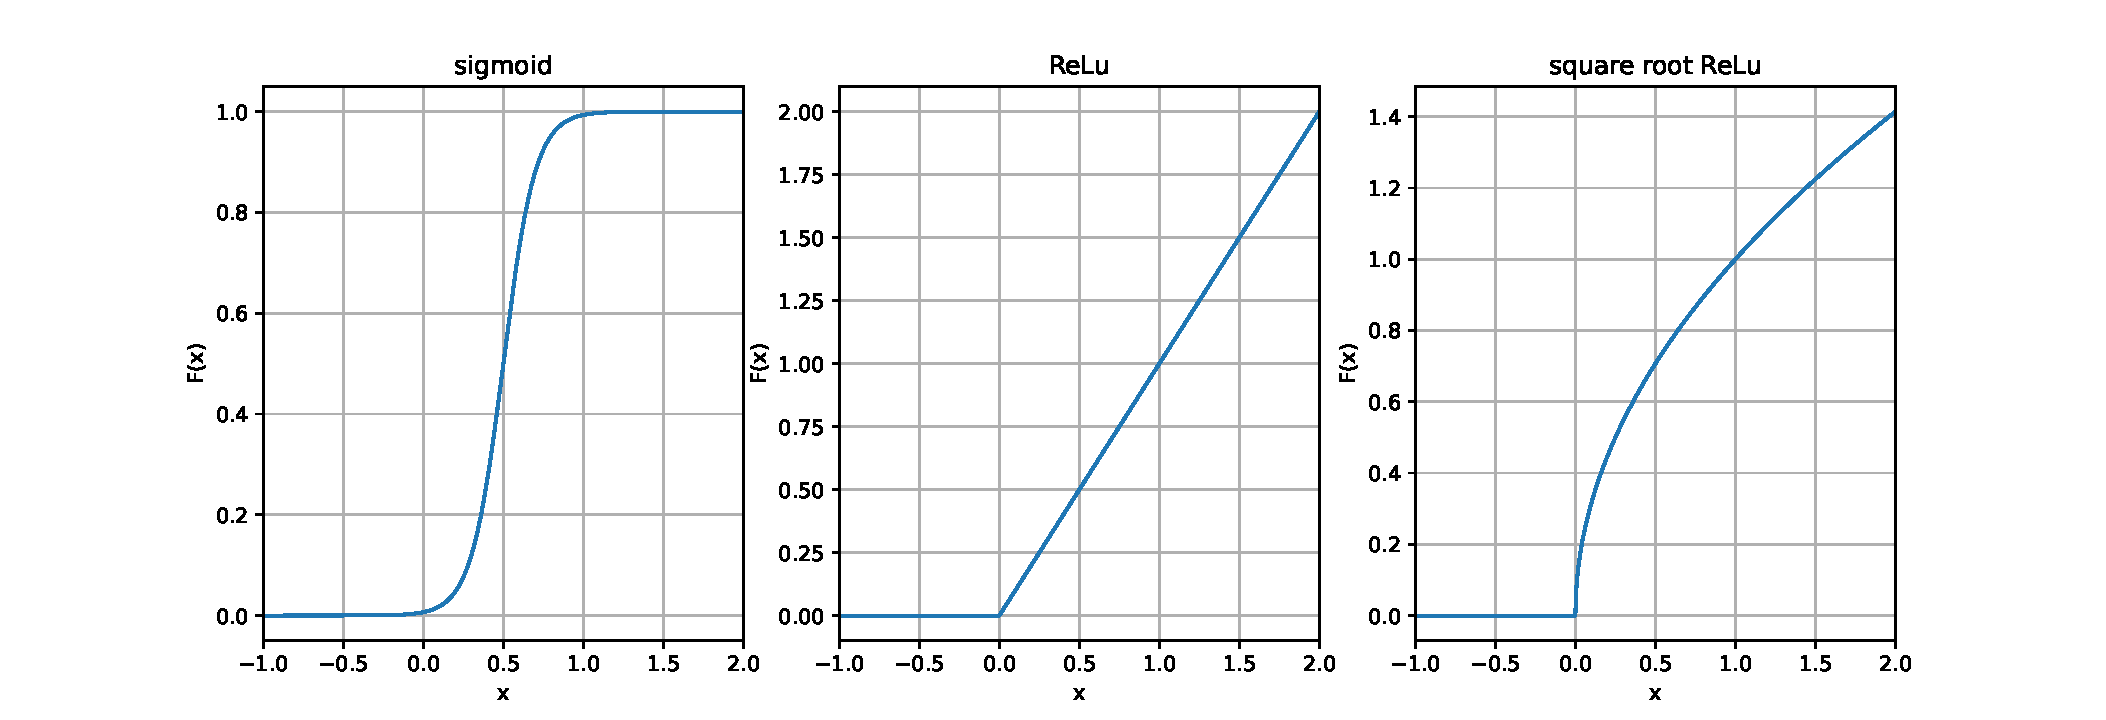
\includegraphics[width=1\linewidth]{figures/gains}\\
    \caption{Gain function profiles.
    \label{fig:plot_gains}}
\end{figure}

The equations of a couple of connected firing rate units the following equations (similar to equation \ref{single_unit_eqn} but with the addition of a connectivity term with strength $w$)
\begin{equation}
    \begin{array}{lcl}
    \tau \cdot \dot{r}_1 & = & -r_1 + S(I + \alpha r_1 - w r_2 - b a_1) \\
    \tau \cdot \dot{r}_2 & = & -r_2 + S(I + \alpha r_2 - w r_1 - b a_2) \\
    \tau_a \cdot \dot{a}_1 & = & -a_1 + r_1 \\
    \tau_a \cdot \dot{a}_2 & = & -a_2 + r_2.
    \end{array}
    \label{coupled_eqn}
\end{equation}
This crossed coupling term represents the commissural projections found in swimming animals.

\subsection*{Metrics}
To evaluate the model we provided your the following three metrics of the neural network (stored in the dictionary \fileref{network.py::FiringRateController().metrics} and computed in \fileref{util/metrics.py}):
\begin{itemize}
\item \textbf{frequency}: returns the frequency of the first element of the state array \fileref{network.py::Fi\-ringRateController().state[:,0]}. Use it to compute the frequency of the firing rate variable $r$ of systems \ref{single_unit_eqn} and \ref{coupled_eqn}. Internally, the code computed the frequency from the last two threshold crossings of \fileref{network.py::FiringRateController().state[:,0]}.
\item \textbf{amp}: return the amplitude of \fileref{network.py::FiringRateController().state[:,0]}
\item \textbf{sync}: computes a mesure of synchronization for the coupled units (only valid for system \ref{coupled_eqn}). It has values between 0 and 1, where 0/1=inphase synchronization and 0.5=antiphase synchronization.
\end{itemize}

\subsection*{Numerical integration}
In all simulations, we consider only steady-state dynamics (we exclude transient dynamics) and starting from uniformly random initial conditions in all the system's variables. Simulations can be run using two options:
\begin{itemize}
\item \fileref{util.run\_open\_loop.py::run\_simulation(pars)} - runs a single simulation with simulation parameters specified by the \fileref{simulation\_parameters.py::SimulationParameters()} class.
\item \fileref{util.run\_open\_loop.py::run\_multiple(pars\_list)} - runs multiple simulation in parallel using your computer cores from a list of \fileref{simulation\_parameters.py::SimulationParameters()} classes. Use this function to speed up computations in parameter searches.
\end{itemize}



%%%%% Exercises

\section*{Exercises}

\subsection*{4.a Implement the equations of a single firing rate neural controller unit with
 sigmoid gain function and adaptation (equation \ref{single_unit_eqn} and equation \ref{sigmoid_eq}). This network represents the
 central pattern generator in a single hemisegment in a fish or lamprey (as seen in the lectures).
 Run systematic simulations when varying the self-excitation strength $\alpha \in [0,3]$. How is the behavior of the single unit changing? Is this in line with what we know from the lamprey/fish literature?}


\subsection*{4.b Implement the equations for the coupled firing rate controllers \ref{coupled_eqn} with sigmoid
 gain function, no self-excitation and $w=2$ (low inhibition). What does the output looks
 like? Run a systematic parameter sweep varying the input $I \in [0,10]$. What dynamical behavior can the model generate
 for different values of $I$?
}


\subsection*{4.c Repeat the same study as in Exercise 4.b (same parameters and specifications as in
Exercise 4.b) for higher levels of inhibition $w=3.8$. Do new states emerge when varying $I \in [0,10]$ as in exercise 4b?}




\subsection*{4.d Repeat the same study as in Exercise 4.b/c replacing the sigmoid gain by a ReLU
 function (equation \ref{ReLu_eq}) and by the square root of the ReLu gain (equation \ref{SReLu_eq}). Discuss the simlarities/differences with these previous cases.}




\subsection*{4.e Now study the role of excitatory and inhibitory coupling. What happens to the pair if the weight
 are now excitatory ($w<0$)? Run a parameter sweep of $w \in [-2,5]$ Use the sync metric to describe your findings. Experiments revealed the existence of crossed inhibitory connections are dominant for explaining the swimming rhythm. Do your results corroborate these findings? }


\end{document}